% research (8-10 pages)
\chapter{Проучване}
\hfill
\section{Терминали}
От библиотеката се изисква създадаването на текстови потребителски интерфейси,
което зависи от средата, в която се изпълнява програмата. Разгледани са 
възможните среди без съсредоточаване в детайлите. \\
        \subsection{Телетайп терминал - TTY}
                Този вид терминал се нарича така, поради сходността си с 
                телеграфния апарат. На фигура \ref{fig:hw_tty} е показана
                блокова схема на принцип на работа на TTY терминал.
                Потребителят пише на хардуерния терминал, който е свързан към
                UART (универсален асинхронен приемник и предавател) на 
                компютъра. Операционната система на компютъра съдържа UART 
                драйвер, който управлява физическото предаване на байтове. 
                "Дисциплината на линията" определя командите за редактиране на 
                терминала - например изтрии линия, препечатай линия, 
                изтрий дума. \\
        
                \begin{figure}[H]
                        \centering
                        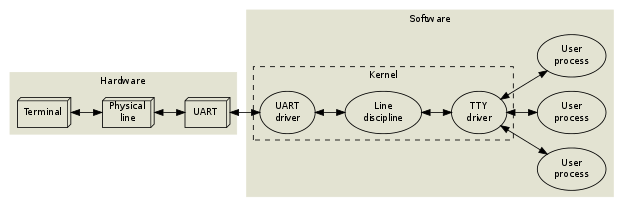
\includegraphics[
                                angle=0,
                                origin=center,
                                width=\linewidth
                        ]{images/teletype_block_diagram.png}
                        \caption{Принцип на работа на хардуерен TTY}
                        \label{fig:hw_tty}
                \end{figure}
                \vspace{10mm}

        \subsection{Псевдотелетайп терминал - PTY}
                Фигура \ref{fig:linux_tty} постига същия резултат като фигура
                \ref{fig:hw_tty}, като разликата е, че хардуерен терминал вече
                не се използва. Linux ядрото използва софтуерно реализиран 
                краен автомат, който емулира същите функционалности. \\
                \cite{tty}

                \begin{figure}[H]
                        \centering
                        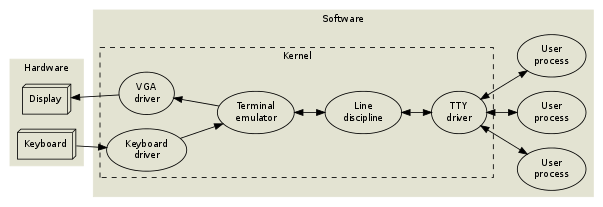
\includegraphics[
                                angle=0,
                                origin=center,
                                width=\linewidth
                        ]{images/linux_tty_block_diagram.png}
                        \caption{Принцип на работа на PTY}
                        \label{fig:linux_tty}
                \end{figure}
                \vspace{10mm}


        \subsection{Терминален емулатор}
                Терминалните емулатори използват PTY подсистемата, но за 
                разлика от PTY работят на ring 3 (потребителско пространство). 
                Това ниво на абстракция добавя много повече гъвкавост, но и 
                усложнява имплементацията си, защото един PTY може да се отвори
                в друг PTY. \\
                \indent{}
                Тази гъвкавост води до разлики в терминалните емулатори. Част 
                от тези, които са програмирани преди въвеждането на ISO 6429, 
                не го имплементират, а други имплементират разширени CSI кодове
                \\

\section{Контролни символи}
        Контролните символи, също наричани непечатни, нямат графично 
        представяне, а се използват за управление на устройства и предаване на 
        данни. POSIX стандартът дефинира само осем контролни символа, от които 
        по-често използваните са:
        \begin{itemize}
                \item \large \textbackslash 0 - край на символен низ 
                \item \large \textbackslash n - нов ред
                \item \large \textbackslash t - табулация
                \item \large \textbackslash r - връщане на каретата
        \end{itemize}
        \vspace{10mm}

        \subsection{ANSI контролна последователност}
                ANSI кодовете могат да въздействат на поведението на терминала,
                като променят позицията на курсура, цвета на фона и символите, 
                стилизирането на шрифта или други настройки. \\

                Структурата на всички ANSI кодове е следната: \\
                CSI [байтове на режима] n1;n2... [междинни байтове] финален
                байт \\ 

                ANSI последователността винаги започва с CSI и приключва с
                финален байт. Байтовете на режима могат да бъдат в обхват от
                '0' (0x30) до '?' (0x3f), а междинните байтове в обхват от ' '
                (0x20) до '/' (0x2f). Числата n1, n2, ... не са задължителни и,
                ако стойността им не е посочена, се приемат за 0 или 1 в 
                зависимост от операцията, която ще се изпълни заради ANSI кода. 

                Въпреки че е позволено наличието на повече от един междинен 
                байт и байт на режима, това не се ползва.


                \subsubsection{Идентификатор на контролна последователност 
                (CSI)}
                        Преамбюл, с който се разпозначва началото на ANSI кода.
                        Има големина 2 байта, като започва с ESC символ (0x1b) 
                        и "[" (0x5b) \\

\section{Преглед на съществуващи TUI библиотеки}
        \vspace{10mm}
        \subsection{ncurses}
                ncurses е най-използваната библиотека за управление на 
                терминали в UNIX-подобни среди, позволяваща създаване на 
                приложения с текстов потребителски интерфейс. \\

                С ncurses програмистите не трябва да се грижат за използването 
                на правилните контролни символи при различните терминали. 
                Библиотеката предоставя и абстракция за логическо отделение на
                компоненти - прозорци. Прозорците се съпоставят с координатите 
                на терминала, като всеки прозорец представлява масив от 
                символи, в който програмистът може да промени външния вид на 
                прозореца. \\

                Една от най-силните страни на ncurses е съвместимостта на
                библиотеката. Тя може да работи във всякакви среди при 
                всякакви условия \\

                \begin{figure}[H]
                        \centering
                        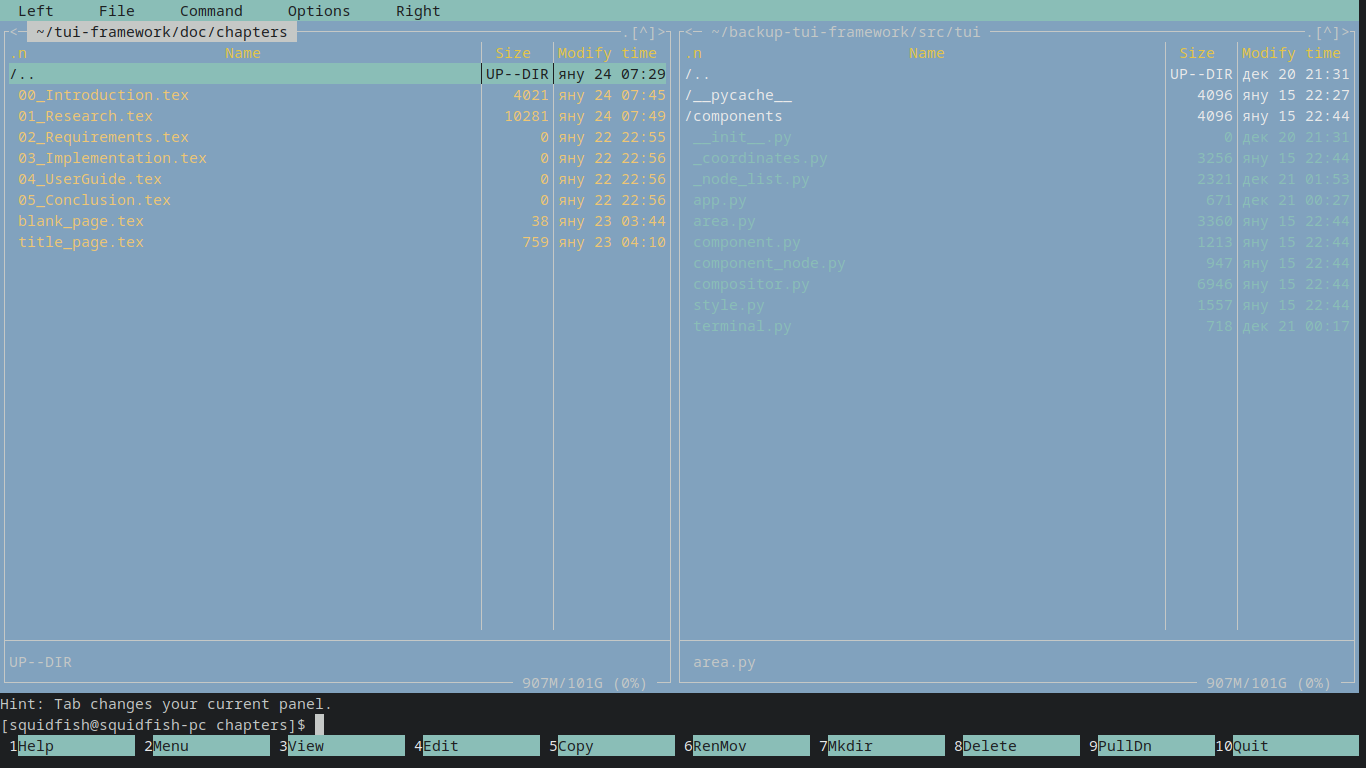
\includegraphics[
                                angle=0,
                                origin=center,
                                width=\linewidth
                        ]{images/ncurses_preview.png}
                        \caption{Midnight Commander - файлов мениджър написани 
                        с ncurses}
                        \label{fig:ncurses_preview}
                \end{figure}
                \vspace{10mm}

        \subsection{Textual}
                Понастоящем Textual е авангардна библиотека за създаване на
                модерни текстови потребителски интерфейси. \\

                Textual взема вдъхновение от уеб разработката. В 
                Библиотеката нивото на абстракция е много по-високо отколкото 
                при ncurses. Използват се компоненти, които са подредени в 
                дървовидна структура и силно наподобяват HTML елементи. 
                Компонентите могат да се стилизрат със CSS. Има поддръжка на 
                мишка и могат да се създават плавни анимации с над 60 кадъра в 
                секунда (в зависимост от терминалния емулатор). \\

                \begin{figure}[H]
                        \centering
                        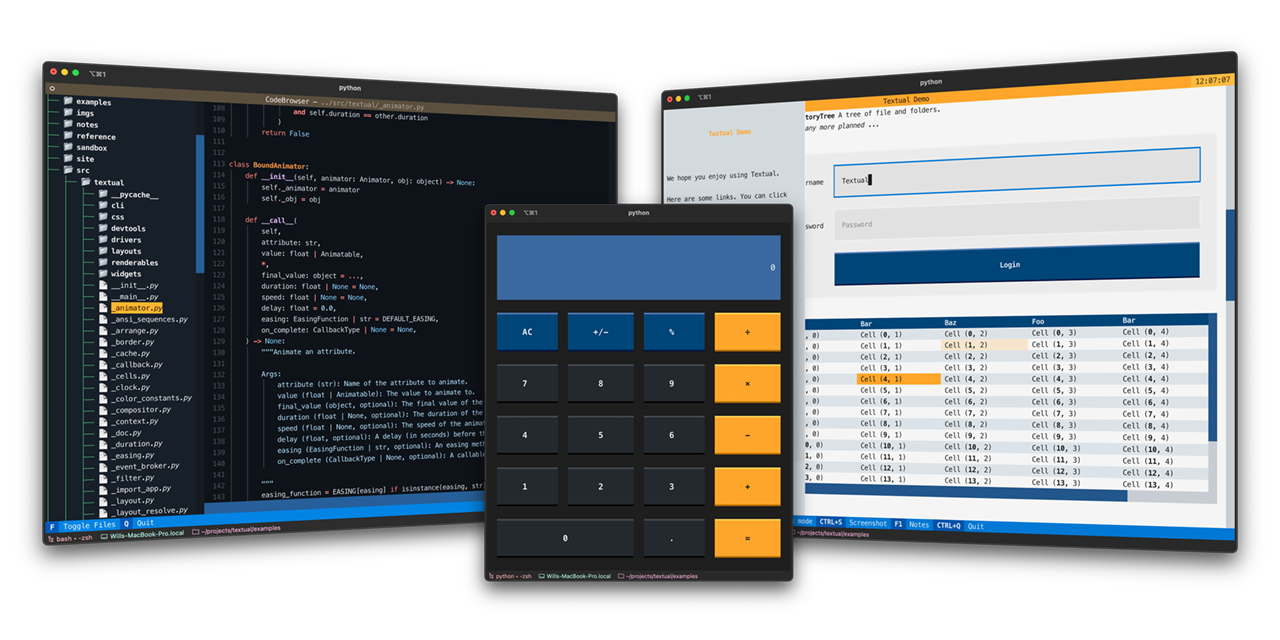
\includegraphics[
                                angle=0,
                                origin=center,
                                width=\linewidth
                        ]{images/textual_preview.png}
                        \caption{Примерни приложения написани с Textual}
                        \label{fig:textual_preview}
                \end{figure}
                \vspace{10mm}
